\chapter{Architecture}
\label{chp:Architecture}

This chapter presents an overview of the architecture of a platform that facilitates the construction of interoperable, reusable, and uniform model management languages, as envisioned in Chapter \ref{chp:Analysis}. This platform is hereafter referred to as \emph{Epsilon}, standing for Extensible Platform for Specification of Integrated Languages for Model Management. 

Describing the architecture also involves making and presenting several high level decisions concerning the organization and structure of the system which will later guide the design and implementation phases. Moreover, it involves identifying the desired quality attributes the architecture should exhibit as well as the mechanisms through which those qualities are achieved (tactics) \cite{SEI}.

The chapter is organized as follows. In Section \ref{sec:Architecture.QualityAttributes}, the desired quality attributes of the architecture are discussed. In Section \ref{sec:Architecture.ArchitecturalTactics}, the main architectural tactics employed for achieving the identified quality attributes are presented. Then, Section \ref{sec:Architecture.ArchitecturalOverview} provides a high-level overview of the architecture and Sections \ref{sec:Architecture.EMC} - \ref{sec:Architecture.DevelopmentTools} provide more details about the individual layers of the architecture and their purpose.

\section{Quality Attributes}
\label{sec:Architecture.QualityAttributes}

Quality attributes are the desired characteristics of the system \cite{SEI}. They can be divided into two major groups: system and business qualities. System qualities refer to the structural and operational aspects of the system and according to the visibility from a user perspective, they can be further separated into observable and unobservable attributes \cite{SEI}. Observable system qualities include among others usability, performance, availability, testability while unobservable attributes include modifiability, portability etc. Business qualities refer to characteristics of the system that are relevant to the business context in which it is developed. Therefore, this category includes attributes such as total cost and time-to-market.

It is important to identify the quality attributes early in the architectural process as they will drive the organization and the structure of the system. In this section, the desirable attributes are identified and classified according to their importance in the context of the system.

\subsection{System quality attributes}

\subsubsection{Modifiability/Extensibility}
The main targets against the which platform is designed are extensibility and modifiability. The motivation for this is that little work has been previously reported on designing platforms of integrated programming languages similar to the one proposed in the context of this thesis. Therefore, it is anticipated that the construction of diverse task-specific languages atop the platform, will likely introduce changes in the platform itself so that it can accommodate similar requirements of different task-specific languages in a consistent, uniform and integrated manner.

\subsubsection{Usability}
The primary aim of providing task-specific languages for different model management tasks is to make it easier for the users to automate specific tasks by using a dedicated focused syntax and a supporting runtime that automates the uninteresting and error-prone parts of each individual task. In this sense, usability is inherently a primary concern of the proposed approach. Also to obtain feedback from external users, as part of the testing and evaluation methodology as discussed in Section \ref{sec:Analysis.ResearchMethodology}, the architecture must provide development tools, that enable users to easily compose and execute model management programs.

\subsubsection{Performance}
In the context of this thesis, the performance of the platform and the languages built atop it is not a primary concern - particularly if it is to be achieved by compromising extensibility or modifiability. However, to be usable, model management programs should generally run in a reasonable amount of time for small and medium-sized models.

\subsection{Business quality attributes}

\subsubsection{Total cost}
Although this is not a commercial project, its budget can be counted in terms of time. In this sense, and since this is a project with many possible extensions, the total design and development time should be kept within balance with the available time and resources.

\section{Architectural Tactics}
\label{sec:Architecture.ArchitecturalTactics}

Tactics are mechanisms that are used in order to achieve the desired quality attributes. As mentioned in \cite{SEI}, \textit{a tactic is a design decision that influences the control of a quality attribute response}. In this section, the tactics used to achieve the quality attributes identified in the previous section are presented.

\subsection{Maintenance of semantic coherence}
Maintaining semantic coherence among the modules of a layer allows the localization of changes and prevention of ripple effects. Therefore, when a change is required, the scope of the change is clearer and narrower. Moreover, when there are expected changes, assigning clear responsibilities to modules and packages will make it easier to perform the alterations without violating the overall architectural decisions and with minimum restructuring and redesign.

\subsection{Separate interface from implementation}
Separating interface from the implementation allows user interface developers and designers to modify the interface in order to achieve enhanced usability without having to propagate the changes into the implementation layer. It is obvious that this tactic enhances modifiability as well.

\subsection{Information hiding}
Limiting visibility to the minimum possible level reduces coupling and enhances modularity. Moreover, it allows for substitution of components with other that provide the same interface.

\subsection{Deferring binding time}
Use of configuration files delays the binding time from compile to execution and allows the user to extend the behaviour of the system without intervening with the source code. Moreover, use of interfaces allows component replacement without modifications to the rest of the source code.\\

\noindent Based on the identified quality attributes and architectural tactics, the remainder sections present an architectural overview of the platform.

\section{Architectural Overview}
\label{sec:Architecture.ArchitecturalOverview}

This section provides a high-level overview of the layers of the proposed architecture and discusses the role of each layer in the overall architecture as well as its relationships to other layers. Chapters \ref{chp:Infrastructure} - \ref{chp:Workflow} refine this abstract architecture into a detailed design that contains sufficient detail to construct a prototype implementation of the platform.

The basis of the architecture of Epsilon, displayed in Figure \ref{fig:EpsilonArchitecture}, is the Model Connectivity layer. This layer enables languages of the platform to access models of diverse technologies and metamodels in a uniform manner. Atop it, the Core Language layer provides a common set of features needed by task-specific model management languages. On top of the Core Language layer, the Task Specific Languages Layer contains a number of task-specific languages that address the tasks of intra and inter-model validation, model comparison, model merging, in-place and model-to-model transformation and model-to-text transformation. The Workflow layer provides support for assembling and coordinating complex model management workflows, and the Development Tools layer contains the tooling through which end-users can specify, debug and execute model management operations. In the following sections, the role of each individual layer is discussed further discussed.

\begin{figure}
	\centering
		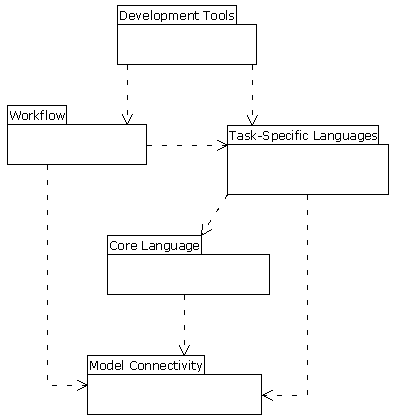
\includegraphics{images/EpsilonArchitecture}
	\label{fig:EpsilonArchitecture}
	\caption{Overview of the architecture of Epsilon}
\end{figure}

\section{The Model Connectivity Layer}
\label{sec:Architecture.EMC}

As discussed in Section \ref{sec:LiteratureReview.MetamodellingArchitectures}, many metamodelling technologies are currently being used to define modelling languages and models. As Epsilon should not be restricted to a particular metamodelling technology or metamodel, a key purpose of the Epsilon Model Connectivity (EMC) layer is to provide a set of facilities through which model management programs will be able to uniformly access and modify models of diverse technologies. Such facilities include:

\paragraph{Loading and persisting models} Models are typically persisted in the file-system, databases or dedicated repositories. EMC is responsible for providing a uniform interface through which technology-specific implementations can define the loading and persistence mechanisms that a particular technology employs.

\paragraph{Type-related operations} During a model management operation it is often necessary to retrieve all the model elements of a particular type or to retrieve the type of a given model element. To abstract away from the diverse type-system implementations in different technologies EMC is responsible for providing a uniform interface for performing type-related operations.

\paragraph{Obtaining and setting values of model element properties} Similarly, modelling technologies provide different implementations for obtaining and setting the values of properties/features (i.e. attributes, references) of model elements. To enable the overlying languages to interact with models of diverse technologies uniformly, EMC provides a uniform interface for retrieving and modifying values of properties of model elements.

\paragraph{Transactions} In case a model management operation fails for some reason (such as an unanticipated exception), there is a risk that models it manages are left in an inconsistent state. To address this issue modelling technologies are increasingly providing support for atomic transactions that can be committed or rolled back on demand - similarly to transactions in relational databases. While not all modelling technologies provide such features yet, EMC provides an interface for managing transactions from languages that use it.\\

\noindent The detailed design of the Model Connectivity layer is presented in Section \ref{sec:Design.EMC}.

\section{The Core Language Layer}
\label{sec:Architecture.EOL}
The purpose of this layer is to provide an extensible and reusable core language, hereafter referred to as the Epsilon Object Language (EOL), which accommodates common facilities of task-specific model management languages. Such facilities include:

\paragraph{Model navigation and querying} This layer is responsible for providing a uniform mechanism for querying and navigating models.

\paragraph{Model modification} A number of model management tasks such as model transformation, refactoring and merging, predominantly update models. To avoid diverse implementations of model modification features in different task-specific languages, EOL provides a uniform set of such features that can be reused by higher order languages.

\paragraph{Access to multiple models} Since the majority of model management tasks needs to access more than one model simultaneously, EOL provides mechanisms that support this functionality.

\paragraph{Statement sequencing and grouping} Sequencing and grouping statements allow developers to disentangle complicated, nested queries making them easier to read and debug.

\paragraph{Reusable operations} To enable reuse between different model management programs, EOL is responsible for providing support for reusable libraries of operations which can be invoked by any language of the platform.

\paragraph{Transactions} As the Model Connectivity layer provides support for transactions, the task-specific languages should also be able to manage transactions programmatically. EOL provides the necessary constructs for this purpose.

\paragraph{Bridge with native code} In some cases, the user of the object language (or a language built atop it) may need to perform an activity which is clearly outside the scope of model management (e.g. to connect to a database server) or a task at which the language is not very efficient at (e.g. to perform complex mathematical computations). To perform such tasks EOL provides support for invoking code written in the programming language in which EOL itself is defined (e.g. Java). This tactic is typical in language construction to avoid dead ends without duplicating functionality from a lower-level language. For example, Java can invoke C code, using JNI \cite{JNI}, and C can invoke Assembly code.

\noindent The detailed design of the Core Language layer is presented in Section \ref{sec:Design.EOL}.

\section{The Task-Specific Languages Layer}
\label{sec:Architecture.TaskSpecificLanguages}

The Epsilon Object Language layer summarised above has been introduced to enable definition of a number of languages, each addressing a specific model management task with little overlap between each other. Each task-specific language in this layer defines its own syntax which however reuses the syntax and facilities provided by EOL. This section briefly discusses the aim and scope of each language in the layer.

\paragraph{Epsilon Transformation Language (ETL)} ETL enables users to specify algorithms that can transform a set of input models to a set of output models of potentially different metamodels.

\paragraph{Epsilon Comparison Language (ECL)}
The purpose of this language is to enable users to specify algorithms that compare elements of two models to establish correspondences between them.

\paragraph{Epsilon Merging Language (EML)} The aim of EML is to enable users to specify how two models should be merged into a third one given a set of correspondences (calculated using ECL or otherwise)

\paragraph{Epsilon Validation Language (EVL)} EVL provides the means to express constraints over model elements which, when evaluated, can reveal inconsistencies in or between models.

\paragraph{Epsilon Wizard Language (EWL)} While ETL targets the problem of expressing batch transformations that transform entire models to other metamodels, EWL enables users to specify interactive in-place model transformations.

\paragraph{Epsilon Generation Language (EGL)} The purpose of EGL is to enable users to generate textual artefacts such as code and documentation from models.

\noindent The detailed design of the Task Specific Languages layer is presented in Chapter \ref{chp:TaskSpecificLanguages}.

\section{The Workflow Layer}
\label{sec:Architecture.Workflow}

As already discussed, in many occasions, a model management process involves more than one distinct steps. For instance, to generate SQL code from a UML model the process would involve validating the UML model, transforming it into a Database model that is more closely related to the target domain using a model-to-model transformation and then generating the SQL code using a model-to-text transformation. The Workflow layer provides support for assembling and executing such model management workflows from individual tasks implemented with languages of the Epsilon platform. The workflow layer provides the following facilities:

\paragraph{Common Model Repository} As discussed in Section \ref{sec:LiteratureReview.Integration}, in the context of a workflow, more than one model management task can be performed on the same models sequentially. Moreover, loading and storing models is a resource and time consuming process, particularly as models grow in size. The aim of the common model repository is to provide centralized management of model loading/storing so that individual model management tasks do not need to load/store the models they operate on themselves. This facility contributes both to decoupling and modularity, and to performance as each model is loaded/stored at most once although it may be used by multiple tasks.

\paragraph{Inter-Task Communication Facility} This facility enables model management programs expressed in different languages of the platform to communicate with each other at runtime by providing a mechanism that allows individual tasks to export variables (for example containing results of complex queries) so that subsequent tasks can reuse them instead of recalculating them.

\noindent The detailed design of the Task Specific Languages layer is presented in Chapter \ref{chp:Workflow}.

\section{The Development Tools Layer}
\label{sec:Architecture.DevelopmentTools}
This layer provides end-user tools for composing, debugging, executing and monitoring individual model management tasks as well as workflows. Provision of user-friendly development facilities is important as it enables external users to experiment with the languages and other facilities of the platform and provide feedback that will contribute to the evolution of the platform.

To achieve uniformity and interoperability with other tools involved in a typical software development process such as compilers, version control systems and graphical editors, the  user-interface should be built atop an extensible integrated development environment (IDE) such as Eclipse \cite{Eclipse}. Building the user interface on such an environment should also deliver productivity and quality benefits as a significant amount of stable and tested functionality, such as support for file management, version control and sophisticated source code editing, can be largely reused.

A detailed discussion on the implementation of the Development Tools layer is presented in Chapter \ref{chp:ReferenceImplementation}.

\section{Chapter Summary}
\label{sec:Architecture.Summary}

This chapter has presented an overview of the architecture of the Epsilon platform that enables development of integrated task-specific languages for model management. It has also discussed the driving quality attributes of the architecture and the architectural tactics that have been employed to achieve them. 

The platform consists of five main layers: the Model Connectivity Layer that enables uniform management of models that are captured in different modelling technologies and metamodels, the Core Language that provides a set of uniform features that are meant to be reused by task-specific languages, the Task-Specific Languages layer that provides a number of languages each of which addresses a distinct model management tasks, the Workflow Layer that provides facilities for integrating individual model management tasks implemented using languages of the platform into coherent workflows and the Development Tools layer that provides end-user tools for composing, executing, debugging and monitoring individual model management tasks and workflows.

The following Chapters \ref{chp:Infrastructure} - \ref{chp:Workflow} refine this abstract architecture into a detailed design that contains sufficient detail to construct a prototype implementation of the platform. 